%%%%%%%%%%%%%%%%%%%%%%%%%%%%%%%%%%%%%%%%%
%
% CMPT 435
% Assignment Two
%
%%%%%%%%%%%%%%%%%%%%%%%%%%%%%%%%%%%%%%%%%

\documentclass[letterpaper, 10pt]{article} 

\usepackage[english]{babel} % English language/hyphenation
\usepackage{graphicx}
\usepackage[lined,linesnumbered,commentsnumbered]{algorithm2e}
\usepackage{listings}
\usepackage{xcolor}
\usepackage{float}
\usepackage{fancyhdr} % Custom headers and footers
\pagestyle{fancyplain} % Makes all pages in the document conform to the custom headers and footers
\usepackage{lastpage}
\usepackage{url}
\usepackage{multirow}

\definecolor{codegreen}{rgb}{0,0.6,0}
\definecolor{codegray}{rgb}{0.5,0.5,0.5}
\definecolor{codepurple}{rgb}{0.58,0,0.82}
\definecolor{backcolour}{rgb}{0.95,0.95,0.92}

\lstset{       
    language=c++,
    backgroundcolor=\color{backcolour},   
    commentstyle=\color{codegreen},
    keywordstyle=\color{magenta},
    numberstyle=\tiny\color{codegray},
    stringstyle=\color{codepurple},
    basicstyle=\ttfamily\footnotesize,
    breakatwhitespace=false,         
    breaklines=true,                 
    captionpos=b,                    
    keepspaces=true,                 
    numbers=left,                    
    numbersep=5pt,                  
    showspaces=false,                
    showstringspaces=false,
    showtabs=false,                  
    tabsize=2                    
}

\fancyhead{} % No page header
\fancyfoot[L]{} % Empty left footer
\fancyfoot[C]{page \thepage\ of \pageref{LastPage}} % Page numbering for center footer
\fancyfoot[R]{}

\renewcommand{\headrulewidth}{0pt} % Remove header underlines
\renewcommand{\footrulewidth}{0pt} % Remove footer underlines
\setlength{\headheight}{0pt} % Customize the height of the header

%----------------------------------------------------------------------------------------
%	TITLE SECTION
%----------------------------------------------------------------------------------------

\newcommand{\horrule}[1]{\rule{\linewidth}{#1}} % Create horizontal rule command with 1 argument of height

\title{	
   \normalfont \normalsize 
   \textsc{CMPT 435 - Fall 2024 - Dr. Labouseur} \\[10pt] % Header stuff.
   \horrule{0.5pt} \\[0.25cm] 	% Top horizontal rule
   \huge Assignment Two -- Searching and Hashing \\     	    % Assignment title
   \horrule{0.5pt} \\[-0.25cm] 	% Bottom horizontal rule
}

\author{Tyler DeLorey \\ \normalsize tyler.delorey1@marist.edu}

\date{\normalsize\ November 1st, 2024}

\begin{document}
 
\maketitle % Print the title

%----------------------------------------------------------------------------------------
%   CONTENT SECTION
%----------------------------------------------------------------------------------------

% Reset figure numbering to include section number
\renewcommand{\thefigure}{\thesection.\arabic{figure}}

\vspace{-5em}
\tableofcontents

\section{Introduction}
\subsection{Changes from First Assignment}

\noindent
Before I explain what I did for this assignment, I want to explain the differences I made between this assignment and the first assignment. Like before, I used C++. I used some code from the last assignment in this one, including Makefile, Node.h, some functions in Sorts.h, and some sections of code from main.cpp. All of Makefile is the same as previously, except for the compiler flags. I added a flag "-Wno-c++11-extensions" to suppress warnings dealing with C++11 extensions, as shown below in Figure 1.1.

\begin{figure}[H]
  \centering
  \lstinputlisting[firstline=4, firstnumber=4, lastline=5]{Makefile} % Makefile
  \caption{Makefile Flag Changes}
  \label{fig:figure1.1}
\end{figure}

\noindent
Of course, I also had to change the header files to match the files used for this assignment, as shown below in Figure 1.2. These were all the changes made in Makefile.

\begin{figure}[H]
  \centering
  \lstinputlisting[firstline=13, firstnumber=13, lastline=14]{Makefile} % Makefile
  \caption{Makefile Header File Changes}
  \label{fig:figure1.2}
\end{figure}

\noindent
Node.h remains almost the exact same as it was in the previous assignment. However, I had to change the type of data that was stored. Before, each Node had a character stored as its data because I was dealing with pushing and enqueuing each character onto a Stack and Queue respectively. Now, for hashing with chaining (which will be explained more in Section 4), I need to have the entire magic item name as the data, instead of each of its letters as its own Node.

\begin{figure}[H]
  \centering
  \lstinputlisting[firstline=13, firstnumber=13, lastline=14]{Node.h}
  \label{fig:figure1.3-part1}
\end{figure}

\vspace{-2em}
\begin{figure}[H]
  \centering
  \lstinputlisting[firstline=20, firstnumber=20, lastline=24]{Node.h}
  \caption{Node.h File Changes}
  \label{fig:figure1.3-part2}
\end{figure}

\noindent
The functions that I used in Sort.h that came from Sorts.h from Assignment 1 were shuffle, partition, and quickSort. As I will explain in the following subsections, I needed a way to both shuffle and sort the array, so I took my implementations of shuffle and quickSort and copied them over to here. Absolutely no code was changed when copying over, except I renamed the "quickSort" function to "sort" just to make it easier to read.

\vspace{1em}

\noindent
The code I copied from main.cpp were things like file reading and using the vector data type in order to store the magic items. Things I added to main.cpp will be addressed further through this entire document.

\subsection{Choosing 42 Random Items}
\noindent
For my implementation of linear and binary search, I only wanted to search for just 42 items out of the 666 in the magic items array. I wanted to choose those 42 items randomly in a very straightforward way. Figure 1.4 below shows how I managed to do this. 

\begin{figure}[H]
  \centering
  \lstinputlisting[firstline=17, firstnumber=17, lastline=18]{main.cpp}
  \label{fig:figure1.4-part1}
\end{figure}

\vspace{-2em}
\begin{figure}[H]
  \centering
  \lstinputlisting[firstline=44, firstnumber=44, lastline=53]{main.cpp}
  \caption{Randomly Choosing 42 Items (main.cpp)}
  \label{fig:figure1.4-part2}
\end{figure}

\noindent
In order to do this, I called the shuffle function from Sort.h to shuffle the magic items array (Line 46). Then, I just took the first forty two items in the magicItems array and put them in another array called randomItems (Lines 47-50). I used a constant called ITEM\_COUNT to store the number 42 (Line 17). This constant also defines the size of the randomItems array (Line 18). Changing the value of this constant changes how many values will be run through the searches. Also, it is important to notice how the magicItems array uses the vector datatype (from Assignment 1) and the randomItems uses a normal C++ array. I did this because the size of the randomItems array is known before its declaration, while the size of the magicItems vector isn't technically known beforehand because the values are being read from a file. It doesn't actually change anything technical in the code because both of them are treated as arrays.

\subsection{Sorting}
\noindent
To perform a binary search, the entire array needs to be sorted. The sort that I use for the array is Quick Sort, as explained earlier. I chose this sort over the others because it has a time complexity of $O(n * log(n))$, which is faster than Selection Sort and Insertion Sort, which have time complexities of $O(n^2)$. The reason why I chose Quick Sort over Merge Sort is because Quick Sort is a in-place sort, meaning the algorithm doesn't need any more than a constant extra amount of space to perform. Above in Figure 1.4 shows when I called the sort function to sort the magicItems array (Line 53). 

\section{Linear Search}
\setcounter{figure}{0} % Reset figure counter

\subsection{Introduction}
\noindent
Linear Search is a type of search that goes through a collection of items one by one until finally it is find or it is not. In the case of this assignment, the item will always be found, but in general, if the item isn't found, the search algorithm will iterate through the entire array. Figure 2.1 below shows the linear search function being called in main.

\begin{figure}[H]
  \centering
  \lstinputlisting[firstline=55, firstnumber=55, lastline=62]{main.cpp} 
  \caption{Iterating Array and Linear Searches (main.cpp)}
  \label{fig:figure2.1}
\end{figure}

\noindent
The search starts out by iterating through the randomItems array (Line 57). Then, each iteration, the linear search function is called to find each random item (randomItems[i]) in the magicItems array (Line 59). Then, the number of comparisons to find the random item is printed (Line 60) and the variable to calculate the average is incremented by the number of comparisons (Line 61). The average count will be further discussed later in this section.

\subsection{Implementing Linear Search}
\noindent
My implementation of linear search is found in the Search.h file. Figure 2.2 below shows how the linear search was implemented in my program.

\begin{figure}[H]
  \centering
  \lstinputlisting[firstline=10, firstnumber=10, lastline=30]{Search.h} 
  \caption{Implementing Linear Search (Search.h)}
  \label{fig:figure2.2}
\end{figure}

\noindent
The function aims to find the target string in the myItems array. The function starts off my initializing the comparison number (Line 14) and the size of the array (Line 16). The function then loops through the array one by one in order to find the target item (Line 19). It starts at the beginning of the array, at index 0, and keep iterating throughout the array until it finds the item or until the last index and the item isn't found (but like mentioned earlier, because of how the program is set up, the item will always be found, however the program in theory handles the cases where it isn't found). If the item at that index in the array is the target item, the program will break (Lines 23-26) and then return the comparison number (Line 29).

\subsection{Printing Average for Linear Search}
\noindent
To get accurate results from the linear search, I found the average amount of comparisons for the linear searches I performed on the 42 items. Figure 2.3 below shows how I accomplished this.

\begin{figure}[H]
  \centering
  \lstinputlisting[firstline=4, firstnumber=4, lastline=4]{main.cpp} 
  \label{fig:figure2.3-part1}
\end{figure}

\vspace{-3em}
\begin{figure}[H]
  \centering
  \lstinputlisting[firstline=21, firstnumber=21, lastline=21]{main.cpp} 
  \label{fig:figure2.3-part2}
\end{figure}

\vspace{-3em}
\begin{figure}[H]
  \centering
  \lstinputlisting[firstline=64, firstnumber=64, lastline=66]{main.cpp} 
  \caption{Finding Average Count for Linear Search (main.cpp)}
  \label{fig:figure2.3-part3}
\end{figure}

\noindent
By the end of the loop shown in Figure 2.1 of Section 2.1 (Lines 57-62), the "avg" variable will be the sum of all comparisons that the linear search performed on the 42 random items, due to its incrementation every iteration on Line 61. In order to find the average from this sum, this number must be divided by the number of inputs. In this case, there were 42 inputs because the linear search was executed 42 times, once on each item. This division operation is shown on Line 65 (back in Figure 2.3). Line 66 prints out the average number of comparisons that the linear search performs. 

\vspace{1em}

\noindent
Because I want the overall average to print up to two decimal places, I had to use the fixed manipulator and the setprecision function, which are available in the iomanip C++ library (Line 4). Used together allow the programmer to set the decimal precision used for an output. The fixed manipulator ensures that the output uses fixed-point notation, meaning the number of digits after the decimal point is fixed. This is different from floating-point notation, where the decimal point can "float" depending on the magnitude of the number. The setprecision function is set to 2 because I want the number to display up to 2 decimal places. Since it is fixed-point notation, it will always display 2 decimal places no matter the magnitude of the number.

\vspace{1em}

\noindent
Notice how the "avg" variable is declared and initialized as a float (Line 21). This is because the final average count will show precision up to 2 decimal places, so an integer would not be a valid data type to store this information. 

\subsection{Results for Linear Search}
\noindent
The table below shows the results of 10 runs of the program. Each result in the table is the average comparison count of 42 results, so there are technically 420 total linear searches in the entire table.

\begin{table}[H]
    \centering
    \begin{tabular}{|c|}
        \hline
        \textbf{Linear Search Results} \\ \hline
        296.79 \\ 
        363.05 \\ 
        303.12 \\ 
        373.31 \\ 
        303.64 \\ 
        362.74 \\ 
        361.33 \\ 
        357.60 \\ 
        317.19 \\ 
        350.93 \\ \hline
    \end{tabular}
    \caption{Linear Search for an Array of Size 666}
    \label{tab:tab1}
\end{table}

\noindent
To actual use this data and interpret it into something that it actually meaningful, it is important to the note the time complexity of linear search. Linear search is $O(n)$ since the worst case scenario iterates through the entire array once if the target element is at the last index, or it's not in the array at all. In this case, $n = 666$ because there are 666 items in the entire magic items array. The best case of linear search is $O(1)$ since there is a chance where the first item that is looked at is the target item (the item at index 0 is the target item). The average case of linear search is $O(n / 2)$ because on average, the item will be found towards the middle of the array. However, the average case time complexity is technically also $O(n)$ because asymptotic notation ignores constants. 

\vspace{1em}

\noindent
When looking at the table results, I will be using $O(n / 2)$ to get more accurate results. In this case, as mentioned previously, n = 666, so the average result should be around 333. In the table of the linear search results, all of those values are very close to 333, proving that the average case for linear search is $O(n / 2)$. This can be further proven by taking the average of all the averages, which is $338.97$. This number is extremely close to 333. Most likely, if this process keeps continuing, and more linear searches are completed, it will get closer and closer to the number 333, or $n/2$.

\section{Binary Search}
\setcounter{figure}{0} % Reset figure counter

\subsection{Introduction}
\noindent
Binary Search is a type of search that divides a sorted array or collection of items into halves repeatedly until eventually the item is found, or it is not. In the case of this assignment, like with linear search, the item will always be found. Figure 3.1 below shows the binary search function being called in main.

\begin{figure}[H]
  \centering
  \lstinputlisting[firstline=68, firstnumber=68, lastline=77]{main.cpp} 
  \caption{Iterating Array and Binary Searches (main.cpp)}
  \label{fig:figure3.1}
\end{figure}

\noindent
The code in main is very similar to the code that was used for Linear Search (view Figure 2.1 to see the comparison). The only aspect added to the Binary Search code is setting the "avg" variable back to 0 (Line 69). Because this takes place after the linear search code, the average count needs to be reset. Then, like linear search, it starts out by iterating through the randomItems array (Line 72). Each iteration, the binary search function is called to find each random item (randomItems[i]) in the magicItems array (Line 74). Then, the number of comparisons to find the random item is printed (Line 75) and the variable to calculate the average is incremented by the number of comparisons (Line 76). It is important to notice that I am using the same "random" items as I did for the linear search. The randomItems array has not been altered at all.

\subsection{Implementing Binary Search}
\noindent
My implementation of binary search is found in the Search.h file. Figure 3.2 below shows how the binary search was implemented in my program.

\begin{figure}[H]
  \centering
  \lstinputlisting[firstline=32, firstnumber=32, lastline=64]{Search.h} 
  \caption{Implementing Binary Search (Search.h)}
  \label{fig:figure3.2}
\end{figure}

\noindent
The function aims to find the target string in the myItems array using recursion. 

\vspace{1em}

\noindent
I used a very similar implementation regarding the parameters of this function like I did for the mergeSort and quickSort functions in Assignment 1. I didn't want to have any extra parameters in the original call of the function in main.cpp (Line 74 of Figure \ref{fig:figure3.1} shows the program calling binarySearch(magicItems, randomItems[i]) with no extra parameters). I wanted to do this to increase readability for the main function, instead of also including the comparison count, the begin index, and the end index parameters in the function call. To do this, I had to use default parameters. A problem came with this because I couldn't set the default parameter for the variable "end" to myItems.size() - 1 because an error would occur stating that myItems may not appear in that context. Like before, I think the error occurs because myItems wouldn't be accessible whenever the function was declared because it isn't static. Setting the "end" variable to INT\_MIN as a default parameter seemed to do the trick again. All I had to do was check if that variable was equal to INT\_MIN, and if it was, it would be changed to equal myItems.size() - 1 (Lines 38-41 of Figure 3.2) because that's the last index of the whole array.

\vspace{1em}

\noindent
Now, moving on to the actual binary search. To ensure the function has only one exit point, I created a variable returnValue to hold the return value (Line 42). There is only one return to this function, located on Line 63. To divide the array into halves, I calculated the middle index for the current range of indices (myItems[begin] ... myItems[end]) being searched (Line 43). Each recursive call will do one comparison, so the comparison count is incremented (Line 45). Then, there is a block of if-else statements:

\begin{itemize}
    \item The first if statement checks whether or not the calculated midpoint is the target item, meaning it has been found, or if there are no more items to search, meaning the target is not in the array (Line 48). The second case shouldn’t occur in this program since I’m only searching for values known to be in the list. In either case, the function sets returnValue to the comparison count (Line 50) and eventually returns this value (Line 63).
    \item The second if statement handles the case where the target item has a smaller ASCII value than the midpoint (Line 53). Because the array is already sorted, this means there’s no need to search the upper half of the array. The function recursively calls itself, narrowing the search to the lower half from the beginning index up to, but not including, the midpoint (Line 55). The returned comparison count is passed back up to ensure each call in the recursion gets the correct count (Line 63).
    \item The else statement runs only if the target item has a larger ASCII value than the midpoint (Line 58). Here, there’s no need to search the lower half of the array. The function recursively calls itself to search the upper half, from the midpoint + 1 to the end index, again excluding the midpoint (Line 60). As with the previous cases, the comparison count returned from this function call is passed back up on Line 63, allowing the recursion to keep track of the correct comparison count.
\end{itemize}

\subsection{Printing Average for Binary Search}
\noindent
To get accurate results from the binary search, I found the average amount of comparisons for the binary searches I performed on the 42 items. Figure 3.3 below shows how I accomplished this.

\begin{figure}[H]
  \centering
  \lstinputlisting[firstline=79, firstnumber=79, lastline=81]{main.cpp} 
  \caption{Finding Average Count for Binary Search (main.cpp)}
  \label{fig:figure3.3}
\end{figure}

\noindent
The functionality of this section of the program is the exact same as linear search. The "avg" variable will be the sum of all comparisons that the binary search performed on the 42 random items, due to its incrementation every iteration on Line 76 of Figure 3.1. Then, to find the average, the sum is divided by the ITEM\_COUNT (Line 80). Like linear search, I had to use the fixed manipulator and the setprecision function to print the overall average up to two decimal places (Line 81).

\subsection{Results for Binary Search}
\noindent
The table below shows the results of 10 runs of the program. Each result in the table is the average comparison count of 42 results, so there are technically 420 total binary searches in the entire table. Also, note that the binary search function will be executed more than 420 times since the function uses recursion to divide the array into halves.

\begin{table}[H]
    \centering
    \begin{tabular}{|c|}
        \hline
        \textbf{Binary Search Results} \\ \hline
        8.45 \\ 
        8.52 \\ 
        8.69 \\ 
        8.40 \\ 
        8.17 \\ 
        8.64 \\ 
        8.76 \\ 
        8.62 \\ 
        8.69 \\ 
        8.50 \\ \hline
    \end{tabular}
    \caption{Binary Search for an Array of Size 666}
    \label{tab:tab2}
\end{table}

\noindent
It is important to the note the time complexity of binary search. Binary search is $O(log(n))$. This is because every iteration, the array is being divided into half. Dividing an input size of $n$ like this results in logarithmic time, just like how Merge Sort and Quick Sort both do dividing, and a portion of their time complexity consists of $log(n)$ (there is no conquering like there is in Merge Sort or Quick Sort, which is why binary search time complexity is just $O(log(n))$ and not $O(n * log(n))$ like those sorts). More specifically, the time complexity for binary search should be $O(\log_2 n)$ since it is being divided into halves (2 halves, hence the log is base 2). However, since asymptotic notation ignores constants, it is just $O(log(n))$. In this case, $n = 666$ because there are 666 items in the entire magic items array. 

\vspace{1em}

\noindent
The best case of binary search is $O(1)$ since there is a chance where the first item that is looked at is the target item (the item at the mid point is the target item). The average case of binary search is also approximately $O(log(n))$ because it is very similar to the worst case scenario. The search may need to go on until there is just one element left. 

\vspace{1em}

\noindent
As mentioned previously, n = 666, so the average result should be around $\log_2 666 \approx 9.38$. In the table of the binary search results, all of those values are close to 9.38, and they are all actually smaller. The reason why the calculated result isn't 100\% accurate is because it is difficult to calculate the average case for binary search because the results can vary so much.

\section{Hash Table}
\setcounter{figure}{0} % Reset figure counter

\subsection{Introduction}
\noindent
The next type of search completed in this assignment uses a hash table. A hash table is a data structure mostly used for fast lookup times. An input is passed through a hashing function that returns a (mostly) unique index. This index is used to store the item. When searching for an item in a hash table, all that needs to be done is put that input into the hashing function, and the value will be found (or not) in close to constant time (time complexity of the hash table will be explained later).

\vspace{1em}

\noindent
My implementation of a hash table is shown below in Figure 4.1.

\begin{figure}[H]
  \centering
  \lstinputlisting[firstline=7, firstnumber=7, lastline=12]{Hash.h}
  \caption{Hash Table (Hash.h)}
  \label{fig:figure4.1}
\end{figure}

\noindent
My hash table is an array of pointers to Nodes (Line 12). The array is of size 250, as determined by the constant set on Line 11. The Node class is the exact same as the one from the previous assignment, and like I explained in Section 1.1, the only thing that is different is the data type being stored is now a string instead of a single character.

\vspace{1em}

\noindent
My implementation of a hash table uses hashing with chaining to handle collisions. If two separate inputs get passed into the hash function and they return the same index (which does happen), there needs to be some way to handle the collision, otherwise data will be overwritten and lost. One way to handle collision is hashing with probing. This is when the collision object is moved to the next index in the array. This can cause even more problems since the array has limited space and there could be some item that needs to go in that next index, and the problem may keep repeating itself. This is why I implemented hashing with chaining. When two or more items are assigned the same index, they're stored at a linked list at that index. More about the linked lists will be explained with the hashPut function. 

\vspace{1em}

\noindent
Below is how I implemented the hash table functions in main.

\begin{figure}[H]
  \centering
  \lstinputlisting[firstline=83, firstnumber=83, lastline=94]{main.cpp}
  \caption{Hash Table Searches and Iterating Array (main.cpp)}
  \label{fig:figure4.2}
\end{figure}

\noindent
I'm not going to explain this section of the program in extreme detail since most of it is extremely similar to both the linear search and the binary search. However, there are a couple differences. The most notable one is that the hash table in Hash.h needs to be loaded with the data from the magicItems array. I do this by calling the hashPut function I created (Line 84), which will be explained in detail in Section 4.3. Next, the average variable is reset (Line 87). Then with each iteration of the loop, the hash search function called hashGet is called to find each random item (randomItems[i]) in the hash table (Line 91). Then, the number of comparisons to find the random item is printed (Line 92) and the variable to calculate the average is incremented by the number of comparisons it took (Line 93). Like before, these are the same "random" items used for both previous searches.

\subsection{hashIndex}
\noindent
The first function to explain in Hash.h is the hash index function because it's the backbone for the functionality of the hash table. This function takes an input and correlates it with some index value. Below is my implementation of the function.

\begin{figure}[H]
  \centering
  \lstinputlisting[firstline=14, firstnumber=14, lastline=28]{Hash.h}
  \caption{hashIndex (Hash.h)}
  \label{fig:figure4.3}
\end{figure}

\noindent
The function begins by declaring and initializing a variable named total (Line 18). The value of this variable may get to be very large, so I made it unsigned so it could store even more values since it doesn't need space for negative numbers. My hash function calculates the index based on adding the ASCII value of each character in the string (Lines 22-25). Something unique I added to this function is multiplying the total by 13 every iteration (Line 24). Multiplying by a prime number helps introduce the idea of the values becoming more spread out and "random". This helps reduce the chances of collision.

\vspace{1em}

\noindent
After the total is calculated, it has to correspond with an index in the hash table. In order to make sure the total is not larger than the amount of indices in the table (which it most definitely will be), I use the modulo operator. Doing the total \% HASH\_TABLE\_SIZE operation (Line 27) makes sure that the value returned from the function will be from 0 - HASH\_TABLE\_SIZE - 1. In this case, since the hash table size is 250, the range of possible values returned would be from 0-249, which  correspond with the bounds of the hash table.

\vspace{1em}

\noindent
Increasing the size of the hash table will definitely reduce the amount of collisions of indices in the hash table, however it would require a lot more space. There is a trade-off between space and time when it comes to algorithms, especially when talking about hash tables. 

\subsection{hashPut}
\noindent
The hash put function is the function that actually loads the hash table with the magic items. This was the function called in main (Line 84 in Figure 4.2). Below is my implementation of this function.

\begin{figure}[H]
  \centering
  \lstinputlisting[firstline=30, firstnumber=30, lastline=46]{Hash.h}
  \caption{hashPut (Hash.h)}
  \label{fig:figure4.4}
\end{figure}

\noindent
The function begins by initializing a size variable to be the size of the myItems (magicItems) array (Line 33). It also declares and initializes a variable called "value" that will eventually store the index of the hash table the item will be put into (Line 34). A variable called "curItem" is also declared, which will store the name of the current item being worked with in the loop (Line 35). The loop at Line 37 loops through the entire array. Each iteration, curItem will be set to the current item (Line 39) and the item will be passed through the hashIndex function explained back in Section 4.2. The index returned from that function will be set in the "value" variable (Line 40).

\vspace{1em}

\noindent
Now it is time to deal with the linked list at that specific index. Each index in the hash table array has a linked list. My implementation of the linked list within the index has the new Node be inserted at the "head" of the list. First, the new Node was created with its data being the name of the current item being dealt with (Line 42). Then, the new Nodes next pointer will be set to the current Node at that correct index (43). This is essentially the former "head" of the linked list. Lastly, the new Node will be set to that index of the hash table (Line 44), making the new Node the "head" of the linked list. The reason why I decided to insert the new Node at the beginning of the linked list is because I wanted it to run in constant time, or $O(1)$. Inserting the new Node at the end of the linked list (without a pointer to the "tail") would be $O(n)$, where $n$ represents the amount of Nodes in the linked list at that index in the hash table. Once the loop is complete, all the magic items will be in the hash table.

\subsection{hashGet}
\noindent
The hashGet is the function that searches through the hash table for the target item. Below is my implementation of this search function.
\begin{figure}[H]
  \centering
  \lstinputlisting[firstline=48, firstnumber=48, lastline=68]{Hash.h}
  \caption{hashGet (Hash.h)}
  \label{fig:figure4.5}
\end{figure}

\noindent
The function starts off by declaring and initializing the comparison number variable (Line 52). Then, exactly like the hashPut function, a variable called "value" stores the index of the hash table the item should be in (Line 53). On this line, the target item is passed through the hashIndex function. So, technically, if the item was in the hash table, it would be at that index returned by the hashIndex function. This means there is no reason to search any other index of the hash table. This also counts as a comparison for the comparison count, so that value is incremented (Line 55).

\vspace{1em}

\noindent
Because now the program only looks at that calculated index in the hash table, it will only iterate through the linked list at the index (Line 58-65). Each iteration of this loop increases the comparison count (Line 60). Then, the program checks if the current Node's data is the target item (Line 61). If it is, the search is successful and then the program breaks out of the loop (Line 63) and returns the comparison number (Line 67). In the case of this program, like explained a thousand times beforehand, the target item will always be found because of how it was set up. However, in a case where it isn't found, the loop will end once the pointer becomes NULL.

\subsection{hashUnload}
\noindent
C++ doesn't have any automatic garbage collection. This makes it very easy for memory leaks to occur. Because of this, there needs to be some sort of way that the hash table can be unloaded since new objects (Nodes) were being created that were never deleted. First of all, the unload function call is at the end of main, as shown below in Figure 4.6.

\begin{figure}[H]
  \centering
  \lstinputlisting[firstline=100, firstnumber=100, lastline=101]{main.cpp}
  \caption{hashUnload Function Call (main.cpp)}
  \label{fig:figure4.6}
\end{figure}

\noindent
Now that the function call is established, it is time to dive into the specifics of how this function works. The implementations of the hashUnload function and its helper function (hashUnloadIndex) are shown below in Figure 4.7

\begin{figure}[H]
  \centering
  \lstinputlisting[firstline=70, firstnumber=70, lastline=91]{Hash.h}
  \caption{hashUnload and hashUnloadIndex (Hash.h)}
  \label{fig:figure4.7}
\end{figure}

\noindent
The hashUnload function iterates through the hash table, one index at a time (Lines 84-90). If there is at least one Node at the current index (Line 86), then that Node, and all other Nodes that may be in the linked list at the index, need to be deleted. This is where the hashUnloadIndex function is called (Line 88).

\vspace{1em}

\noindent
The hashUnloadIndex actually does the deleting from memory. This is also a recursive function. If the given parameter Node is NULL, then it returns back to the hashUnload function to continue its iterations (Lines 73-76). If it's not, the function will be called again and again until it reaches the "tail" of the linked list (Line 77). Once it reaches the tail, it will delete the Node and then the Node before it, and the one before that, etc (Line 78). It starts by deleting the Node at the end of the linked list since the Node's next pointers would be pointing at garbage values if we delete the first Node in the linked list. Therefore, the other Nodes would be lost in memory.

\vspace{1em}

\noindent
The time complexity of the hash table search will all be explained in Section 4.7, but since the unload function is complete separate, I would like to explain that here. The time complexity of the unload function is $O(n)$, where $n$ represents the amount of Nodes in the hash table. In this case, $n = 666$. This is because the program has to visit every Node in order to delete it, which makes the time complexity of the unload $O(n)$.

\subsection{Printing Average for Hash Table Search}
\noindent
To get accurate results from the hash table searches, I found the average amount of comparisons for the table searches I performed on the 42 items. Figure 4.8 below shows how I accomplished this.

\begin{figure}[H]
  \centering
  \lstinputlisting[firstline=96, firstnumber=96, lastline=98]{main.cpp} 
  \caption{Finding Average Count for Hash Table Search (main.cpp)}
  \label{fig:figure4.8}
\end{figure}

\noindent
The functionality of this section of the program is the exact same as linear search and binary search. The "avg" variable will be the sum of all comparisons that the search performed on the 42 random items, due to its incrementation every iteration on Line 93 of Figure 4.2. Then, to find the average, the sum is divided by the ITEM\_COUNT (Line 97). Again, I had to use the fixed manipulator and the setprecision function to print the overall average up to two decimal places (Line 98).

\subsection{Results for Hash Table Search}
\noindent
The table below shows the results of 10 runs of the program. Each result in the table is the average comparison count of 42 results, so there are technically 420 total hash "gets" in the entire table.

\begin{table}[H]
    \centering
    \begin{tabular}{|c|}
        \hline
        \textbf{Hash Table Search Results} \\ \hline
        3.38 \\ 
        3.05 \\ 
        3.02 \\ 
        3.10 \\ 
        3.57 \\ 
        3.17 \\ 
        3.24 \\ 
        3.57 \\ 
        3.29 \\ 
        3.29 \\ \hline
    \end{tabular}
    \caption{Hash Table Search for an Array of Size 666 and Hash Table Size of 250}
    \label{tab:tab3}
\end{table}

\noindent
It is important to the note the time complexity of hash table lookup. As eluded to earlier, hash table searching is extremely close to constant time, which is $O(1)$. However, the time complexity of hash table lookup is noted at $O(1 + \alpha)$. The 1 represents the "get" comparison, meaning when the hashIndex function is executed to find the correct index to search through. The $\alpha$, or alpha, represents the average chain length, also referred to as the load factor. The average chain length can be calculated by dividing the number of items, or Nodes, in the hash table by the size of the hash table.   

\vspace{1em}

\noindent
For the case of this assignment, the hash table is of size 250, and there are 666 Nodes in the hash table. To find the average chain length, the equation is $666/250 = 2.664$. Now obviously this is just an estimate since it is the AVERAGE chain length. All that needs to be done now is to plug in that number for $\alpha$ in the time complexity, so the time complexity of this specific hash table search is $O(1 + 2.664) = O(3.664)$. All of the values in the table above are very close to 3.664, thus proving that this is the average case.

\subsection{Adjusting Size of Hash Table}
\noindent
What if the size of the hash table was changed? How would this affect the time complexity of the algorithm? The solution to solve these questions is pretty easy to implement, considering I had the HASH\_TABLE\_SIZE constant, which I could change on each run of the program. Here are some comparison number results I got when changing the hash table size. 

\vspace{-1em}
\begin{table}[H]
    \centering
    \begin{tabular}{|c|c|c|}
        \hline
        \textbf{Table size = 25} & \textbf{Table size = 250} & \textbf{Table size = 2500} \\
        \hline
        15.90 & 3.55 & 2.05 \\
        14.07 & 3.57 & 2.17 \\
        14.45 & 3.17 & 2.07 \\
        14.12 & 3.14 & 2.24 \\
        15.83 & 3.76 & 2.10 \\
        \hline
    \end{tabular}
    \caption{Hash Table Comparison Results when Changing Table Size}
    \label{tab:tab4}
\end{table}

\noindent
It is obvious that there is a relationship between the table size of the number of comparisons to do the hash table lookup. To further prove this, I can use the equal mentioned in the last subsection, $O(1 + \alpha)$.

\begin{itemize}
    \item For when the table size is 25, $\alpha$ would be equal to $666/25 = 26.64$, and $26.64 + 1 = 27.64$, meaning the average time complexity is 27.64. The reason why I think this average value is slightly off from the values in the table is because of the hashing function I used to find the correct index. Either way, having less buckets in the hash table means there will be more comparisons on average.
    \item For when the table is 250, as proven in the last subsection, the average time complexity would be 3.664. This is obviously a better result than when the hash table is smaller, but it seems to be worse than the results when the hash table is larger.
    \item For when the table size is 2500, $\alpha$ would be equal to $666/2500 = 0.2664$, and $0.2664 + 1 = 1.2664$, meaning the average time complexity is 1.2664. However, because of my implementation of the Hash.h functions, the minimum amount of comparisons to find an item will always be 2. There must be 1 to find the correct index (the get), and another to see if the head of the linked list at the calculated index is the target item. 
\end{itemize}

\noindent
Like hinted at earlier, though, this is a case of prioritizing time or space. Allocating more space to store a larger hash table means that the lookup times will be faster. However, if the programmer doesn't want to use that much space, they don't have to.

\section{Conclusion}
\setcounter{figure}{0}

\vspace{-1em}
\begin{figure}[H] 
    \centering 
    \fbox{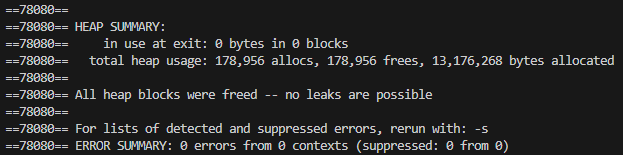
\includegraphics[width=0.98\textwidth]{./imgs/ValgrindOutput.PNG}}
    \caption{Valgrind Output (running command "valgrind ./main")}
    \label{fig:figure5.1}
\end{figure}

\vspace{-1em}
\noindent
In conclusion, this assignment was another great learning experience for me. Implementing linear and binary search was a fun and relaxing experience. Implementing the hash table, especially with unloading it, took me a bit longer to do, but it was still fun. Speaking of unloading the hash table, I used Valgrind a lot to see if the unloading functions were working properly. As seen in Figure 5.1, there were no memory leaks at all, meaning the Nodes were successfully deleted. Valgrind was, again, very useful for me to use. I'm having a great time working in C++.

\end{document}
